%!TEX root = thesis.tex
%-------------------------------------------------------------------------------
\chapter{Extended Nonlocal Games}
\label{chap:extended_nonlocal_games}
%-------------------------------------------------------------------------------

In this chapter, we introduce the \emph{extended nonlocal game} model. This model is a generalization of the nonlocal game model in which the referee now also holds a quantum system provided to it by Alice and Bob at the start of the game. In Section~\ref{sec:the-model-of-extended-nonlocal-games} we shall present the extended nonlocal game protocol, and in Section~\ref{sec:strategies-extended-nonlocal-games}, we define the corresponding strategies that Alice and Bob may adopt during the course of the game. 

The general notion of extended nonlocal games was previously considered by Fritz~\cite{Fritz2012}. In particular, Fritz considered a class of games, called \emph{bipartite steering games}, which are essentially extended nonlocal games in which the referee randomly chooses to ask either Alice or Bob a question. Extended nonlocal games may also be viewed as being equivalent to multipartite steering inequalities, in a similar way to the equivalence between nonlocal games and Bell inequalities. Multipartite steering inequalities and related notions were studied in the papers~\cite{Cavalcanti2015} and~\cite{Sainz2015}. The term ``extended nonlocal game'' along with a treatment more focused in the nonlocal game setting was carried out in~\cite{Johnston2015a}. 

This chapter is based on joint work with Nathaniel Johnston, Rajat Mittal, and John Watrous~\cite{Johnston2015a}

\minitoc

%-------------------------------------------------------------------------------
\section{The extended nonlocal game model}
\label{sec:the-model-of-extended-nonlocal-games}
%-------------------------------------------------------------------------------

Extended nonlocal games are a generalization of nonlocal games in which the \emph{referee also holds a quantum system}, provided to it by Alice and Bob at the start of the game. Similar to an ordinary nonlocal game, one may consider a variety of possible strategies for Alice and Bob in an extended nonlocal game. In particular, there are classes of strategies that are analogous to classical, quantum, commuting measurement, and non-signaling strategies from the nonlocal game model. Further details on how these are adapted for the case of extended nonlocal games will be elaborated on in this chapter. 

An \index{extended nonlocal game}{\emph{extended nonlocal game}} is similar to a nonlocal game in the sense that it is a cooperative game played between two players, Alice and Bob, against a referee. The game begins much like a nonlocal game, with the referee selecting and sending a pair of questions $(x,y)$ according to a fixed probability distribution. Once Alice and Bob receive $x$ and $y$, they respond with respective answers $a$ and $b$. Unlike a nonlocal game, the outcome of an extended nonlocal game is determined by measurements performed by the referee on its share of the state initially provided to it by Alice and Bob. Specifically, Alice and Bob's winning probability is determined by a collection of measurements, $V(a,b|x,y) \in \Pos(\R)$, where $\R = \complex^m$ is a complex Euclidean space with $m$ denoting the dimension of the referee's quantum system---so if Alice and Bob's response $(a,b)$ to the question pair $(x,y)$ leaves the referee's system in the quantum state 
\begin{align}
	\sigma_{a,b}^{x,y} \in \Density(\R),
\end{align}
then their winning and losing probabilities are given by 
\begin{align}
	\biggip{V(a,b|x,y)}{\sigma_{a,b}^{x,y}} \quad \textnormal{and} \quad \biggip{\I - V(a,b|x,y)}{\sigma_{a,b}^{x,y}}.
\end{align}

%Specifically, Alice and Bob's winning probability is determined by an \emph{observable}, $V(a,b|x,y) \in \Herm(\R)$, where $\R = \complex^m$ is a complex Euclidean space with $m$ denoting the dimension of the referee's quantum system---so if Alice and Bob's response $(a,b)$ to the question pair $(x,y)$ leaves the referee's system in the quantum state 
%\begin{align}
%	\sigma_{a,b}^{x,y} \in \Density(\R),
%\end{align}
%then their winning probability will be the real-number value 
%\begin{align}
%	\biggip{V(a,b|x,y)}{\sigma_{a,b}^{x,y}}.
%\end{align}
%In the event where the outcome of an extended nonlocal game results in a binary win or a loss, we may consider the referee to be in possession of a collection of positive semidefinite measurement operators $V(a,b|x,y) \in \Pos(\R)$ instead of Hermitian operators indexed by $(x,y) \in \Sigma$ and $(a,b) \in \Gamma$. In this case, the respective winning and losing probabilities are given by
%\begin{align}
%	\biggip{V(a,b|x,y)}{\sigma_{a,b}^{x,y}} \quad \textnormal{and} \quad \biggip{\I - V(a,b|x,y)}{\sigma_{a,b}^{x,y}}.
%\end{align}
%Extended nonlocal games defined in terms of binary-valued measurements will be the primary type of extended nonlocal game we will consider in this thesis, unless noted otherwise.   

%-------------------------------------------------------------------------------
\section{Strategies for extended nonlocal games} \label{sec:strategies-extended-nonlocal-games}
%-------------------------------------------------------------------------------

%-------------------------------------------------------------------------------
\subsection{Extended nonlocal games and assemblage operators} \label{sec:extended-nonlocal-games-and-assemblage-operators}
%-------------------------------------------------------------------------------

%\comment{In the nonlocal games section in the previous chapter, there is this notion of a correlation operator, denoted as $C((x,a),(y,b))$ for each type of strategy. Introducing this allows one to talk about the sets $\L,\C,\Q$, etc. of correlation operators. This is useful because it motivates and explains what the NPA and extended NPA hierarchies are useful for. A question I have then is whether to: 
%	\begin{itemize}
%		\item Also introduce a correlation operator for extended nonlocal games, and to explicitly define how it looks for each strategy (seems somewhat cumbersome)
%		\item To just refer to the sets of correlation operators for extended nonlocal games as obvious extensions, and perhaps refer to each set as something like $\L^E,\C^E,\Q^E$, where "E" is for extended. 
%		\item To remove the correlation operator definitions in the nonlocal game sections, as perhaps their use in the thesis is not justified for as much space as they take up. 
%	\end{itemize}
%Not entirely sure what the best way to go about this is, but I wanted to note it here, as there seems like there is a bit of a disconnect in terms of how the nonlocal and extended nonlocal games are defined. 
%}

An extended nonlocal game $H$ is defined by a pair $(\pi,V)$, where $\pi$ is a probability distribution of the form 
\begin{align}
	\pi : \SigmaA \times \SigmaB \rightarrow \left[0,1\right]
\end{align}
on the Cartesian product of two alphabets $\SigmaA$ and $\SigmaB$, and $V$ is a function of the form 
\begin{align}
	V : \GammaA \times \GammaB \times \SigmaA \times \SigmaB \rightarrow \Pos(\R), 
\end{align}
for $\SigmaA$ and $\SigmaB$ as above, $\GammaA$ and $\GammaB$ being alphabets, and $\R$ refers to the referee's space. Just as in the case for nonlocal games, we shall use the convention that
\begin{align}
	\Sigma = \SigmaA \times \SigmaB \quad \textnormal{and} \quad \Gamma = \GammaA \times \GammaB
\end{align}
to denote the respective sets of questions asked to Alice and Bob and the sets of answers sent from Alice and Bob to the referee. 

When analyzing a strategy for Alice and Bob, it may be convenient to define a function 
\begin{align}
	K : \GammaA \times \GammaB \times \SigmaA \times \SigmaB \rightarrow \Pos(\R).
\end{align}
We will refer to the function $K$ as an \index{assemblage}{\emph{assemblage}}. The operators output by this function represent the \emph{unnormalized} states of the referee's quantum system when Alice and Bob respond to the question pair $(x,y)$ with the answer pair $(a,b)$. 

%as 
%\begin{align}
%	K(a,b|x,y) = \tr_{\A \otimes \B} \left( \left( \I_{\R} \otimes A_a^x \otimes B_b^y \right) \rho \right)
%\end{align}
%for each $x \in \SigmaA$, $y \in \SigmaB$, $a \in \GammaA$, and $b \in \GammaB$. 

We can however, if we wish, normalize these states by noting that the quantity $\tr\left(K(a,b|x,y)\right)$ refers to the probability with which Alice and Bob answer $(a,b)$ for the question pair $(x,y)$. Assuming that $\tr \left( K(a,b|x,y) \right) > 0$, we define a set of normalized states 
\begin{align} \label{eq:enlg-conditional-states}
	\sigma_{a,b}^{x,y} = \frac{K(a,b|x,y)}{\tr \left( K(a,b|x,y) \right)}
\end{align}
of the referee's system conditioned on this question and answer pair. Note that the function $K$ completely determines the performance of Alice and Bob's strategy for $H$ as it encodes the probability that Alice and Bob obtain answers $a \in \GammaA$ and $b \in \GammaB$ given questions $x \in \SigmaA$ and $y \in \SigmaB$ as
\begin{align}
	\tr \left( K(a,b|x,y)	\right),
\end{align} 
along with the conditional states from equation~\eqref{eq:enlg-conditional-states}. In particular, Alice and Bob's winning probability is represented as 
\begin{align} \label{eq:quantum-winning-probability-kabxy}
	\sum_{(x,y) \in \Sigma} \pi(x,y) \sum_{(a,b) \in \Gamma} \biggip{V(a,b|x,y)}{K(a,b|x,y)}. 
\end{align}

%This may be observed by noting that equation~\eqref{eq:quantum-winning-probability-kabxy} may be written as equation~\eqref{eq:enlg-quantum-winning-probability}, that is
%\begin{align}
%	 &\sum_{(x,y) \in \Sigma} \pi(x,y) \sum_{(a,b) \in \Gamma} \biggip{V(a,b|x,y)}{K(a,b|x,y)} \\
%	 &=\sum_{(x,y) \in \Sigma} \pi(x,y) \sum_{(a,b) \in \Gamma} \biggip{V(a,b|x,y)}{\tr_{\A \otimes \B} \left( \left( \I_{\R} \otimes A_a^x \otimes B_b^y \right) \rho \right)} \\
%	 &=\sum_{(x,y) \in \Sigma} \pi(x,y) \sum_{(a,b) \in \Gamma} \tr \left( V(a,b|x,y) \tr_{\A \otimes \B} \left( \left( \I_{\R} \otimes A_a^x \otimes B_b^y \right) \rho \right) \right)  \label{eq:ip-to-tr-1} \\
%	 &=\sum_{(x,y) \in \Sigma} \pi(x,y) \sum_{(a,b) \in \Gamma} \tr \left( \left(V(a,b|x,y) \otimes A_a^x \otimes B_b^y \right) \rho \right) \label{eq:factor-out-pt} \\
%	 &=\sum_{(x,y) \in \Sigma} \pi(x,y) \sum_{(a,b) \in \Gamma} \biggip{V(a,b|x,y) \otimes A_a^x \otimes B_b^y}{\rho}, \label{eq:ip-to-tr-2} 
%\end{align}
%where in equations~\eqref{eq:ip-to-tr-1} and~\eqref{eq:ip-to-tr-2}, we used the relationship between the inner product and trace operations, and in equation~\eqref{eq:factor-out-pt}, we factor out the partial trace operator from the overall trace. 

%In an extended nonlocal game, for any type of strategy, the output probability distributions produced by Alice and Bob may be described by an \index{extended correlation operator}{\emph{extended correlation operator}}. Such an operator is defined as 
%\begin{align}
%	C^m \in \Lin(\complex^m \otimes \real^{\SigmaA \times \GammaA}, \complex^m \otimes \real^{\SigmaB \times \GammaB}),
%\end{align}
%where $C_{i,j}^m( (x,a),(y,b) )$ is the probability that Alice and Bob output 
%
%\comment{TODO: fill out requirements of extended correlation operator.}

%-------------------------------------------------------------------------------
\subsection{Standard quantum strategies for extended nonlocal games} \label{sec:standard-quantum-strategies-extended-nonlocal-games}
%-------------------------------------------------------------------------------

A \index{standard quantum strategy (extended nonlocal game)}{\emph{standard quantum strategy}} for an extended nonlocal game consists of finite-dimensional complex Euclidean spaces $\U$ for Alice and $\V$ for Bob, a quantum state $\sigma \in \Density(\U \otimes \R \otimes \V)$, and two collections of measurements, 
\begin{align}
	\{ A_a^x : a \in \GammaA \} \subset \Pos(\U) \quad \textnormal{and} \quad \{ B_b^y : b \in \GammaB \} \subset \Pos(\V),
\end{align}
for each $x \in \SigmaA$ and $y \in \SigmaB$ respectively. As usual, the measurement operators satisfy the constraint that 
\begin{align}
	\sum_{a \in \GammaA} A_a^x = \I_{\U} \quad \textnormal{and} \quad \sum_{b \in \GammaB} B_b^y = \I_{\V},
\end{align}
for each $x \in \SigmaA$ and $y \in \SigmaB$. 

When the game is played, Alice and Bob present the referee with a quantum system so that the three parties share the state $\sigma \in \Density(\U \otimes \R \otimes \V)$. The referee selects questions $(x,y) \in \Sigma$ according to the distribution $\pi$ that is known to all participants in the game. The referee then sends $x$ to Alice and $y$ to Bob. At this point, Alice and Bob make measurements on their respective portions of the state $\sigma$ using their measurement operators to yield an outcome to send back to the referee. Specifically, Alice measures her portion of the state $\sigma$ with respect to her set of measurement operators $\{A_a^x : a \in \GammaA\}$, and sends the result $a \in \GammaA$ of this measurement to the referee. Likewise, Bob measures his portion of the state $\sigma$ with respect to his measurement operators $\{ B_b^y : b \in \GammaB \}$ to yield the outcome $b \in \GammaB$, that is then sent back to the referee. At the end of the protocol, the referee measures its quantum system with respect to the measurement $\{ V(a,b|x,y), \I - V(a,b|x,y) \}$. 

\begin{figure}[!htpb] \label{fig:extended-nonlocal-game}
	\begin{center}
		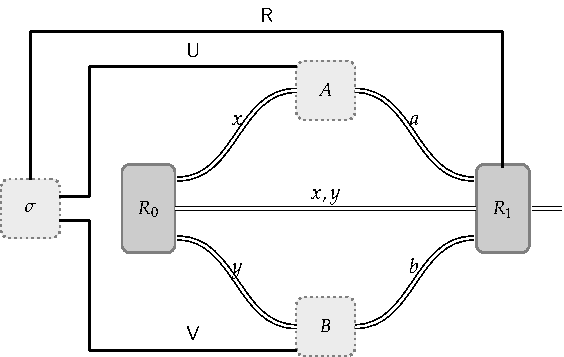
\includegraphics[scale=0.9]{figures/enlg_2.pdf}
	\end{center}
		\caption[A two-player extended nonlocal game.]{A two-player extended nonlocal game. Alice, Bob, and the referee all share a tripartite state, $\sigma \in \Density(\U \otimes \R \otimes \V)$, contained in registers $(\reg{U},\reg{R},\reg{V})$. The referee selects questions $(x,y) \in \Sigma$ according to the probability distribution $\pi$, and sends $x$ to Alice and $y$ to Bob. Upon receiving $x$ and $y$, Alice and Bob respond with answers $a \in \GammaA$ and $b \in \GammaB$. After receiving $a$ and $b$, the referee performs a measurement on its system $\{ V(a,b|x,y), \I - V(a,b|x,y) \}$ to determine the probability with which Alice and Bob win the game.}
\end{figure}

The winning probability for such a strategy in this game $H = (\pi,V)$ is given by 
\begin{align} \label{eq:enlg-quantum-winning-probability}
	\sum_{(x,y) \in \Sigma} \pi(x,y) \sum_{(a,b) \in \Gamma} \biggip{A_a^x \otimes V(a,b|x,y) \otimes B_b^y}{\sigma},
\end{align}  
or equivalently the winning probability for such a strategy is given by 
\begin{align}
	\sum_{(x,y) \in \Sigma} \pi(x,y) \sum_{(a,b) \in \Gamma} \biggip{V(a,b|x,y)}{K(a,b|x,y)},
\end{align}
where the operator $K : \GammaA \times \GammaB \times \SigmaA \times \SigmaB \rightarrow \Pos(\R)$ is a \index{standard quantum assemblage}{\emph{standard quantum assemblage}} operator defined as 
\begin{align}
	K(a,b|x,y) = \tr_{\U \otimes \V} \left( \left( A_a^x \otimes \I_{\R} \otimes B_b^y \right) \sigma \right).
\end{align}
This may be observed by noting that 
\begin{align}
	 &\sum_{(x,y) \in \Sigma} \pi(x,y) \sum_{(a,b) \in \Gamma} \biggip{V(a,b|x,y)}{K(a,b|x,y)} \\
	 &=\sum_{(x,y) \in \Sigma} \pi(x,y) \sum_{(a,b) \in \Gamma} \biggip{V(a,b|x,y)}{\tr_{\U \otimes \V} \left( \left(  A_a^x \otimes \I_{\R} \otimes B_b^y \right) \sigma \right)} \\
	 &=\sum_{(x,y) \in \Sigma} \pi(x,y) \sum_{(a,b) \in \Gamma} \tr \left( V(a,b|x,y) \tr_{\U \otimes \V} \left( \left( A_a^x \otimes \I_{\R} \otimes B_b^y \right) \sigma \right) \right)  \label{eq:ip-to-tr-1} \\
	 &=\sum_{(x,y) \in \Sigma} \pi(x,y) \sum_{(a,b) \in \Gamma} \tr \left( \left( A_a^x \otimes V(a,b|x,y) \otimes B_b^y \right) \sigma \right) \label{eq:factor-out-pt} \\
	 &=\sum_{(x,y) \in \Sigma} \pi(x,y) \sum_{(a,b) \in \Gamma} \biggip{ A_a^x \otimes V(a,b|x,y) \otimes B_b^y}{\sigma}, \label{eq:ip-to-tr-2} 
\end{align}
where in equations~\eqref{eq:ip-to-tr-1} and~\eqref{eq:ip-to-tr-2}, we used the relationship between the inner product and trace operations, and in equation~\eqref{eq:factor-out-pt}, we factor out the partial trace operator from the overall trace. 

For any strategy, there is an equivalent strategy where $\sigma$ is a pure state and the sets of measurements that Alice and Bob possess are projective operators. This can be shown through a two step process. First, either party may purify the state. It makes no difference whether Alice or Bob hold the purification, but for the sake of argument, we assume that Alice purifies the state. Second, the non-projective measurements can be simulated by projective measurements in a standard way that is described by Naimark's theorem~\cite{Paulsen2003}. 


%Observe that for $\Z_0 = \R \otimes \X \otimes \Y$ and for some complex Euclidean space, $\Z_1$, that a purification given by vector $u \in \Z_0 \otimes \Z_1$ satisfying $\tr_{\Z_1}(uu^*) = \rho$ does not change the value from equation~\eqref{eq:enlg-quantum-winning-probability}. Furthermore, it is a consequence of the finite dimensional case of \index{Naimark's theorem}{\emph{Naimark's theorem}} that any strategy for Alice and Bob that makes use of non-projective measurements can be simulated by a projective measurement strategy. 

%Let $\GammaA$ be the alphabet for Alice's outputs, let $\Z_0 = \R \otimes \X \otimes \Y$ and let $\Z_1 = \complex^{\GammaA}$ be a complex Euclidean space with $w \in \Z_1$. Define 
%\begin{align}
%	v = u \otimes w_0 \in \Z_0 \otimes \Z_1 \quad \textnormal{and} \quad \widetilde{A}_a^x = U^* \left( \I_{\A} \otimes E_{a,a} \right) U,
%\end{align}
%where $U \in \Unitary(\X, \X \otimes \Z_1)$ such that 
%\begin{align}
%	w \otimes w_0 = \sum_{a \in \GammaA} \sqrt{A_a^x} w \otimes e_a
%\end{align}
%for all $w \in \X$. It holds that $\widetilde{A}_a^x$ is projective since $\widetilde{A}_a^x = (\widetilde{A}_a^x)^* \widetilde{A}_a^x$ and 
%\begin{align}
%	\widetilde{A}_a^x v = U^* \left( \I_{\X} \otimes E_{a,a} \right) U \left( u \otimes w_0 \right) = U^* \sqrt{A_a^x} u \otimes e_a.
%\end{align}
%A similar argument holds for Bob's measurement operators as well. As Alice and Bob are free to extend the sizes of their complex Euclidean spaces, it follows from the above argument that any strategy making use of non-projective measurements can be simulated by a projective measurement strategy. That is, any strategy for Alice and Bob defined in terms of the $\{ \widetilde{A}_a^x : a \in \GammaA \}$ and $\{ \widetilde{B}_b^y : b \in \GammaB \}$ as defined above yield the same value in equation~\eqref{eq:enlg-quantum-winning-probability}. So, there is no loss in generality in restricting one's attention to projective measurements $\{ A_a^x : a \in \GammaA \}$ and $\{ B_b^y : b \in \GammaB \}$ for Alice and Bob. 

For a given extended nonlocal game $H = (\pi,V)$, we write $\omega^*(H)$ to denote the \index{standard quantum value}{\emph{standard quantum value}} of $H$, which is the supremum value of Alice and Bob's winning probability over all standard quantum strategies for $H$. We may wish to consider the standard quantum value of $H$ when the dimension on Alice's space and Bob's space are equal to $N$, which we denote as $\omega_N^*(H)$. %We can make the assumption that Alice and Bob's spaces are of equal dimension using the same reasoning as in Section~\ref{sec:quantum-strategies-for-nonlocal-games}.

%-------------------------------------------------------------------------------
\subsection{Unentangled strategies for extended nonlocal games} \label{sec:unentangled-strategies-extended-nonlocal-games}
%-------------------------------------------------------------------------------

An \index{unentangled strategy (extended nonlocal game)}{\emph{unentangled strategy}} for an extended nonlocal game is simply a standard quantum strategy for which the state $\sigma \in \Density(\U \otimes \R \otimes \V)$ initially prepared by Alice and Bob is fully separable. Equivalently, there exists an alphabet $\Delta$ and collections of states 
\begin{align}
	\{ \sigma_j^{\reg{U}} : j \in \Delta \} \subseteq \Density(\U), \quad \{ \sigma_j^{\reg{R}} : j \in \Delta \} \subseteq \Density(\R), \quad \textnormal{and} \quad \{ \sigma_j^{\reg{V}} : j \in \Delta \} \subseteq \Density(\V),
\end{align}
and a probability vector $p \in \P(\Delta)$ such that 
\begin{align}
	\sigma = \sum_{j \in \Delta} p(j) \sigma_j^{\reg{U}} \otimes \sigma_j^{\reg{R}} \otimes \sigma_j^{\reg{V}}.
\end{align} 

Note that any unentangled strategy is equivalent to a strategy where Alice and Bob store only classical information after the referee's quantum system has been provided to it. This is because the state that Alice and Bob share between themselves and the referee is fully separable, that is, there are no quantum correlations that may arise between the constituent subsystems held by the parties. Alice and Bob are therefore justified in following a deterministic strategy on their local systems in a similar way that was considered in classical strategies for nonlocal games.  

%XXX
%\comment{TODO: Prove any unentangled strat is equiv to strat where only classical info.}

Furthermore, any such strategy is equivalent to one given by a convex combination of deterministic strategies, in which Alice and Bob initially provide the referee with a fixed pure state $\sigma = uu^* \in \Density(\R)$, and respond to questions deterministically, with Alice responding to $x \in \SigmaA$ with $a = f(x)$ and Bob responding to $y \in \SigmaB$ with $b = g(y)$ for functions $f: \SigmaA \rightarrow \GammaA$ and $g : \SigmaB \rightarrow \GammaB$.

%XXX
%\comment{Write justification for simplifying unentangled and convex combo of deterministic strats.}

For a given extended nonlocal game $H = (\pi,V)$, we write $\omega(H)$ to denote the \index{unentangled value}{\emph{unentangled value}} of $H$, which is the supremum value for Alice and Bob's winning probability in $H$ over all unentangled strategies. It follows by convexity and compactness that this supremum value is necessarily achieved by some deterministic strategy. The unentangled value for such a game is therefore given by
\begin{align} \label{eq:enlg-unentangled-value}
\omega(G) = \max_{f,g} \biggnorm{ \sum_{(x,y) \in \Sigma} \pi(x,y) V(f(x),g(y)|x,y) },
\end{align}
where the maximum is over all functions $f : \SigmaA \rightarrow \GammaA$ and $g: \SigmaB \rightarrow \GammaB$. 

%Note that in the more general case of an extended nonlocal game, the measurements of the referee are Hermitian operators, i.e. $V(a,b|x,y) \in \Herm(\R)$. The spectral norm as it is defined on Hermitian operators is defined in terms of the largest eigenvalue. In other words, we represent the unentangled value for an extended nonlocal game where the measurements of the referee are Hermitian operators as 
%\begin{align} \label{eq:enlg-unentangled-value}
%	\omega(G) = \max_{f,g} \lambda_{\max} \left( \sum_{(x,y) \in \Sigma} \pi(x,y) V(f(x),g(y)|x,y) \right),
%\end{align}
%where $\lambda_{\max}$ refers to the largest eigenvalue and where the maximum is over all functions $f : \SigmaA \rightarrow \GammaA$ and $g: \SigmaB \rightarrow \GammaB$. Again, we will almost exclusively be concerned with the win or lose outcome for extended nonlocal games, but the formulation is mentioned here for completeness. 

% In the more general case for an extended nonlocal game in which the measurements of the referee are Hermitian operators, i.e., $V(a,b|x,y) \in \Herm(\R)$, since we are ranging over all Hermitian operators, the maximum is obtained by considering the largest eigenvalue. In other words, we represent the unentangled value for an extended nonlocal game where the measurements of the referee are Hermitian operators as 
%\begin{align} \label{eq:enlg-unentangled-value}
%	\omega(G) = \max_{f,g} \lambda_{\max} \left( \sum_{(x,y) \in \Sigma} \pi(x,y) V(f(x),g(y)|x,y) \right)
%\end{align}
%where $\lambda_{\max}$ refers to the largest eigenvalue and where the maximum is over all functions $f : \SigmaA \rightarrow \GammaA$ and $g: \SigmaB \rightarrow \GammaB$. 
%%https://arxiv.org/pdf/1501.01571.pdf 2.1.14
%If instead we were just concerned with an extended nonlocal game that consisted of binary outcomes, the measurements may be represented as positive semidefinite operators. In the event where the measurements are given as such positive semidefinite operators, we can restrict our attention to the following expression
%\begin{align}
%\omega(G) = \max_{f,g} \biggnorm{ \sum_{(x,y) \in \Sigma} \pi(x,y) V(f(x),g(y)|x,y) }.
%\end{align}
%%Note that we are justified in taking the norm instead of maximizing the largest eigenvalue 

%-------------------------------------------------------------------------------
\subsection{Commuting measurement strategies for extended nonlocal games} \label{sec:commuting-measurement-strategies-extended-nonlocal-games}
%-------------------------------------------------------------------------------

A \index{commuting measurement strategy (extended nonlocal game)}{\emph{commuting measurement strategy}} for an extended nonlocal game consists of a single (possibly infinite-dimensional) Hilbert space, $\H$, a quantum state $\sigma \in \Density(\R \otimes \H)$, and two collections of measurements, 
\begin{align}
	\{ A_a^x : a \in \GammaA \} \subset \Pos(\H) \quad \textnormal{and} \quad \{ B_b^y : b \in \GammaB \} \subset \Pos(\H),
\end{align}
such that 
\begin{align}
	\sum_{a \in \GammaA} A_a^x = \sum_{b \in \GammaB} B_b^y = \I_{\H}
\end{align}
for all $x \in \SigmaA$ and $y \in \SigmaB$ and that
\begin{align}
	\left[ A_a^x, B_b^y \right] = 0
\end{align}
for all $x \in \SigmaA, y \in \SigmaB, a \in \GammaA,$ and $b \in \GammaB$. 

For an extended nonlocal game, $H = (\pi,V)$, the winning probability for a commuting measurement strategy is given by 
\begin{align}
	\sum_{(x,y) \in \Sigma} \pi(x,y) \sum_{(a,b) \in \Gamma} \biggip{V(a,b|x,y) \otimes A_a^x B_b^y}{\sigma},
\end{align}
or equivalently the winning probability for such a strategy is given by 
\begin{align}
	\sum_{(x,y) \in \Sigma} \pi(x,y) \sum_{(a,b) \in \Gamma} \biggip{V(a,b|x,y)}{K(a,b|x,y)},
\end{align}
where the operator $K : \GammaA \times \GammaB \times \SigmaA \times \SigmaB$ is a \index{commuting measurement assemblage}{\emph{commuting measurement assemblage}} operator defined as 
\begin{align}
	K(a,b|x,y) = \tr_{\H} \left( \left( \I_{\R} \otimes A_a^x B_b^y  \right) \sigma \right).
\end{align}
This may be observed by noting that
\begin{align}
	 &\sum_{(x,y) \in \Sigma} \pi(x,y) \sum_{(a,b) \in \Gamma} \biggip{V(a,b|x,y)}{K(a,b|x,y)} \\
	 &=\sum_{(x,y) \in \Sigma} \pi(x,y) \sum_{(a,b) \in \Gamma} \biggip{V(a,b|x,y)}{\tr_{\H} \left( \left( \I_{\R} \otimes A_a^x B_b^y \right) \sigma \right)} \\
	 &=\sum_{(x,y) \in \Sigma} \pi(x,y) \sum_{(a,b) \in \Gamma} \tr \left( V(a,b|x,y) \tr_{\H} \left( \left( \I_{\R} \otimes A_a^x B_b^y  \right) \sigma \right) \right)  \label{eq:ip-to-tr-1-com} \\
	 &=\sum_{(x,y) \in \Sigma} \pi(x,y) \sum_{(a,b) \in \Gamma} \tr \left( \left( V(a,b|x,y) \otimes A_a^x B_b^y \right) \sigma \right) \label{eq:factor-out-pt-com} \\
	 &=\sum_{(x,y) \in \Sigma} \pi(x,y) \sum_{(a,b) \in \Gamma} \biggip{V(a,b|x,y) \otimes A_a^x B_b^y  }{\sigma}, \label{eq:ip-to-tr-2-com}
\end{align}
where the analysis follows in a similar manner to the case of standard quantum strategies for extended nonlocal games as described in Section~\ref{sec:standard-quantum-strategies-extended-nonlocal-games}. 

The \index{commuting measurement value (extended nonlocal game)}{\emph{commuting measurement value}} of $H$, which is denoted $\omega_c(H)$, is the supremum value of the winning probability of $H$ taken over all commuting measurement strategies for Alice and Bob. 

%Just as with the standard quantum strategy, it may be convenient to define a function $K : \GammaA \times \GammaB \times \SigmaA \times \SigmaB \rightarrow \Pos(\R)$ as 
%\begin{align}
%	K(a,b|x,y) = \tr_{\H} \left( (\I_{\R} \otimes A_a^x B_b^y) \rho \right)
%\end{align} 
%for each $x \in \SigmaA, y \in \SigmaB, a \in \GammaA$, and $b \in \GammaB$. Such a function arising from a commuting measurement strategy is referred to as a \index{commuting measurement assemblage}{\emph{commuting measurement assemblage}}. 

%It is unknown if every commuting measurement assemblage $K$ is induced by a standard quantum strategy---as shown by Fritz~\cite{Fritz2012}, this problem is closely related to the long-standing Connes Embedding conjecture. 

%-------------------------------------------------------------------------------
\subsection{Non-signaling strategies for extended nonlocal games} \label{sec:non-signaling-strategies-extended-nonlocal-games}
%-------------------------------------------------------------------------------

A \index{non-signaling strategy (extended nonlocal game)}{\emph{non-signaling strategy}} for an extended nonlocal game consists of a function
\begin{align}
	K: \GammaA \times \GammaB \times \SigmaA \times \SigmaB \rightarrow \Pos(\R)
\end{align}
such that
\begin{align} \label{eq:enlg-ns-assemblage}
	\sum_{a \in \GammaA} K(a,b|x,y) = \xi_b^y \quad \textnormal{and} \quad \sum_{b \in \GammaB} K(a,b|x,y) = \rho_a^x,
\end{align}
for all $x \in \SigmaA$ and $y \in \SigmaB$ where $\left\{ \xi_b^y : y \in \SigmaB, \ b \in \GammaB \right \}$ and $\left \{ \rho_a^x : x \in \SigmaA, \ a \in \GammaA \right \}$ are collections of operators satisfying 
\begin{align}
	\sum_{a \in \GammaA} \rho_a^x = \tau = \sum_{b \in \GammaB} \xi_b^y,
\end{align}
for every choice of $x \in \SigmaA$ and $y \in \SigmaB$ and where $\tau \in \Density(\R)$ is a density operator. We refer to the function $K$ satisfying equation~\eqref{eq:enlg-ns-assemblage} as a \index{non-signaling assemblage}{\emph{non-signaling assemblage}}. For any extended nonlocal game, $H = (\pi,V)$, the winning probability for a non-signaling strategy is given by
\begin{align}
	\sum_{(x,y) \in \Sigma} \pi(x,y) \sum_{(a,b) \in \Gamma} \biggip{V(a,b|x,y)}{K(a,b|x,y)},
\end{align}
where $K(a,b|x,y)$ is a non-signaling assemblage. The \index{non-signaling value (extended nonlocal game)}{\emph{non-signaling value}} of $H$, which is denoted as $\omega_{\ns}(H)$, is the supremum value of the winning probability of $H$ taken over all non-signaling strategies for Alice and Bob. Note that the supremum is achieved since the set of non-signaling assemblages is compact which implies the that the supremum is achieved. 

%-------------------------------------------------------------------------------
\subsubsection*{Relationships between different strategies and values}
%-------------------------------------------------------------------------------

It is worth noting that the same inequality chain that holds for nonlocal games also holds for extended nonlocal games, 
\begin{align}
	0 \leq \omega(H) \leq \omega^*(H) \leq \omega_c(H) \leq \omega_{\ns}(H) \leq 1. 
\end{align}
Due to the similarity in definitions of strategies, this line of reasoning is nearly identical to that of Section~\ref{sec:relationships-between-different-strategies-and-values}. 

% XXX PARALLEL REP
%%-------------------------------------------------------------------------------
%\section{Parallel repetition for extended nonlocal games} \label{sec:parallel-rep-extended-nonlocal-games}
%%-------------------------------------------------------------------------------
%
%\comment{TODO...}
%
%A natural question in the context of nonlocal games and extended nonlocal games is to ask how they behave under \index{parallel repetition}{\emph{parallel repetition}}. That is, the setting where Alice and Bob play $r$ copies of the original game, $G$, denoted as $G^r$, wherein the referee gives the players $r$ independent and identically distributed pairs of questions simultaneously and expects a response from Alice and Bob for each instance. The referee accepts if and only if all of the $r$ responses satisfy the criteria for the initial game, and rejects otherwise. 
%
%For a game $G=(\pi,V)$, the repeated game $G^r$ proceeds by the referee selecting $r$ questions pairs $(x_1,y_1), \cdots, (x_r,y_r) \in \Sigma_1 \times \ldots \times \Sigma_r$ based on the probability distribution $\pi$ associated to $G$. The referee then sends the questions $x_1, \ldots, x_r$ to Alice and $y_1, \ldots, y_r$ to Bob. The players then return $r$ answer pairs $(a_1,b_1), \ldots, (a_r,b_r) \in \Gamma_1 \times \ldots \times \Gamma_r$ for each question pair. Alice and Bob win the parallel repetition of $G$ if and only if their answers win each of the $r$ instances of $G^r$. 
%
%\begin{figure}[!htpb] \label{fig:extended-nonlocal-game-parallel-repetition}
%	\begin{center}
%		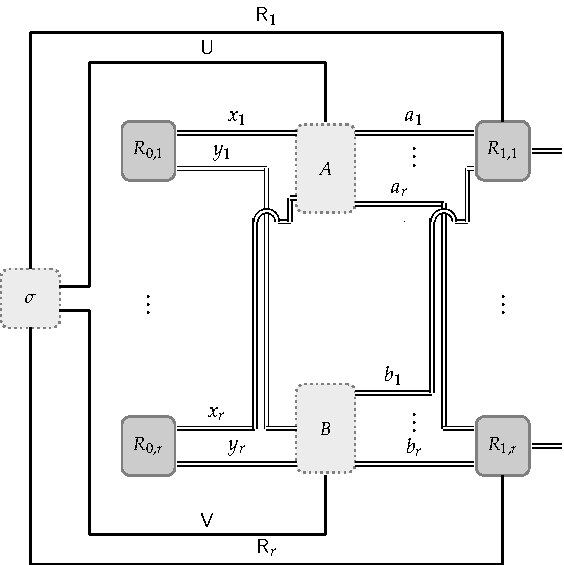
\includegraphics[scale=1.0]{figures/extended_nonlocal_game_parallel_repetition_2.pdf}
%	\end{center}
%		\caption[Parallel repetition of a nonlocal game.]{Parallel repetition of a nonlocal game. Alice and Bob play $r$ copies of the original game where the referee gives the players $r$ independent and identically distributed pairs of questions. The referee accepts if and only if all responses from Alice and Bob in each instance satisfy the criteria for the original game.}
%\end{figure}
%
%One may ask how $\omega(G^r)$ depends on $\omega(G)$ and $r$. It is evident that $\omega(G^r) \geq \omega(G)^r$ since Alice and Bob can simply perform the same strategy in each instance. For any game that has the property $\omega(G) = 1$, it holds that $\omega(G^r) = 1$ for any $r$. One may also wish to ask the question of how $\omega(G^r)$ scales in the event that $\omega(G) < 1$. First note that $\omega(G^r) \leq \omega(G)$. This can be seen since in order for the players to win all instances of the game, they must win the original game, $G$. Note also that $\omega(G)^r \leq \omega(G^r)$ and $\omega(G)^r \leq \omega(G)$. This holds since the players can simply play each game independently with the optimal strategy for the original game. We therefore have the following inequality relationship for the parallel repetition of $G$\
%\begin{align}
%	\omega(G)^r \leq \omega(G^r) \leq \omega(G). 
%\end{align} 
%It may be tempting to conclude that $\omega(G^r) = \omega(G)^r$ for all games, however this was surprisingly disproven~\cite{Fortnow1990, Feige1991, Verbitsky1996, Feige2002}. Specifically in~\cite{Fortnow1990}, Fortnow introduced a game $G$ for which $\omega(G^2) > \omega(G)^2$. This result was later improved by Feige~\cite{Feige1991}, by exhibiting an example of a game where $\omega(G^2) = \omega(G)^2$ with $\omega(G) < 1$.  
%
%In the event where a particular game, $G$, does exhibit $\omega(G^r) = \omega(G)^r$, then we say that the game has the property of \index{strong parallel repetition (perfect parallel repetition)}{\emph{strong parallel repetition}}, also called \emph{perfect parallel repetition}~\cite{Cleve2008} elsewhere in the literature. 